\documentclass[12pt,a4paper]{article}

\usepackage{fontspec}
\usepackage{polyglossia}
\setmainlanguage{russian}
\setotherlanguage{english}
\setmainfont{DejaVu Serif}
\setmonofont{DejaVu Sans Mono}
\usepackage{amsmath, amssymb}
\usepackage{geometry}
\usepackage{graphicx}
\usepackage{booktabs}
\usepackage{longtable}
\usepackage{array}
\usepackage{caption}
\usepackage{hyperref}
\usepackage{listings}
\usepackage{xcolor}

\geometry{left=2.5cm, right=2cm, top=2cm, bottom=2cm}

\lstset{
  basicstyle=\ttfamily\small,
  keywordstyle=\color{blue},
  commentstyle=\color{gray},
  numbers=left,
  numberstyle=\tiny,
  frame=single,
  breaklines=true,
  language=C++
}

\begin{document}

%--- Титульная страница ---
\begin{titlepage}
\begin{center}
{\large Санкт-Петербургский государственный университет}\\[0.3cm]
{\large Математико-механический факультет}\\[0.3cm]
{\large Кафедра физической механики}\\[1.5cm]
{\large Методы измерений и электромеханические системы}\\[1.5cm]
{\LARGE \textbf{Отчёт по лабораторной работе №1}}\\[0.5cm]
{\Large «Многократные прямые измерения физических величин\\
и обработка результатов наблюдений»}\\[0.5cm]
{\large Вариант 1б. Измерение цифровым вольтметром напряжения,\\
задаваемого по стрелочному прибору}\\[2cm]
\end{center}
\begin{flushright}
{\large Выполнил студент:}\\
{\large Ковченко Вениамин Викторович}\\
{\large группа: 24Б5мм}\\[1cm]
{\large Проверил:}\\
{\large к.ф.-м.н., доцент}\\
{\large Кац Виктор Михайлович}\\
\end{flushright}
\vfill
\begin{center}
{\large Санкт-Петербург, 2026~г.}
\end{center}
\end{titlepage}

%--- Содержание ---
\tableofcontents
\newpage

%--- 1. Введение ---
\section{Введение}

\subsection{Цель работы}

Освоить методику многократных прямых измерений физической величины с помощью
цифрового измерительного прибора, а также выполнить статистическую обработку
полученной серии результатов наблюдений.

\subsection{Решаемые задачи}

\begin{enumerate}
\item Провести измерения напряжения на грубой и точной шкалах цифрового
      вольтметра.
\item Проанализировать временну́ю зависимость результатов наблюдений; убедиться
      в отсутствии дрейфа.
\item Построить гистограмму и график плотности распределения $\Delta n / n$;
      оценить дисперсию $\sigma$ по графику.
\item Вычислить среднее значение $\bar{U}$, стандартную погрешность $s$,
      погрешность среднего $s_{\bar{U}}$ и доверительный интервал.
\item Определить погрешность прибора $\omega$ и записать окончательный результат
      согласно выявленной ситуации.
\end{enumerate}

%--- 2. Основная часть ---
\section{Основная часть}

\subsection{Теоретическая часть}

При многократных измерениях физической величины~$X$ получают выборку результатов
отдельных наблюдений
\begin{equation}
  x_1, x_2, \ldots, x_i, \ldots, x_n.
\end{equation}

В качестве наилучшей оценки истинного значения принимается \emph{среднее
арифметическое}:
\begin{equation}
  \bar{x} = \frac{1}{n}\sum_{i=1}^{n} x_i.
  \label{eq:mean}
\end{equation}

\emph{Стандартная погрешность отдельного наблюдения} вычисляется по формуле:
\begin{equation}
  s = \sqrt{\frac{\sum_{i=1}^{n} d_i^2}{n-1}}, \qquad d_i = x_i - \bar{x}.
  \label{eq:s}
\end{equation}

\emph{Погрешность среднего арифметического}:
\begin{equation}
  s_{\bar{x}} = \frac{s}{\sqrt{n}}.
  \label{eq:smean}
\end{equation}

Доверительный интервал с доверительной вероятностью $\alpha$ определяется через
коэффициент Стьюдента $t_{\alpha,n}$:
\begin{equation}
  \varepsilon_\alpha = t_{\alpha,n} \cdot s_{\bar{x}},
  \label{eq:eps}
\end{equation}
и окончательный результат записывается в виде
$x = \bar{x} \pm \varepsilon_\alpha\ (\alpha = \ldots)$.

\emph{Погрешность прибора} цифрового вольтметра задаётся формулой:
\begin{equation}
  S = \pm\!\left(0{,}05 + 0{,}05\cdot\frac{U_K}{U_x}\right)\%,
  \qquad
  \omega = S \cdot U_x \cdot \frac{1}{100},
  \label{eq:omega}
\end{equation}
где $U_K$ — конечное значение используемой шкалы, $U_x$ — измеряемое напряжение.

\subsection{Экспериментальная установка}

Установка состоит из источника постоянного напряжения (УПУ/УИП),
потенциометра (делителя напряжения), стрелочного вольтметра и цифрового
вольтметра. Ручкой потенциометра задавалось напряжение $\approx 0{,}35$~В по
показанию стрелочного прибора. Многократные показания снимались с цифрового
вольтметра.

Схема установки приведена на рис.~\ref{fig:scheme}.

\begin{figure}[h]
  \centering
  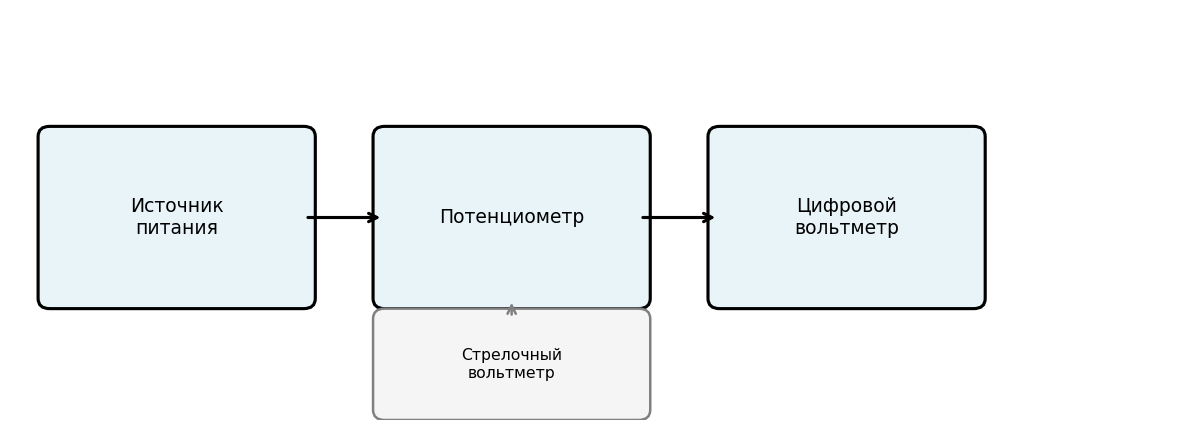
\includegraphics[width=0.55\textwidth]{scheme.png}
  \caption{Блок-схема установки для измерения напряжения цифровым вольтметром}
  \label{fig:scheme}
\end{figure}

\subsection{Обработка данных и обсуждение результатов}

\subsubsection{Исходный код}

Ниже представлен исходный код программы обработки данных (язык Python 3).

\begin{lstlisting}[caption={Функции статистической обработки (C++17)}, label=lst:stat]
// Среднее арифметическое (формула 5 методички)
double mean(const std::vector<double>& x)
{
    double s = 0.0;
    for (double v : x) s += v;
    return s / static_cast<double>(x.size());
}

// Стандартная погрешность отдельного наблюдения (формула 14)
double std_dev(const std::vector<double>& d)
{
    int n = static_cast<int>(d.size());
    double ss = 0.0;
    for (double v : d) ss += v * v;
    return std::sqrt(ss / (n - 1));
}

// Погрешность среднеарифметического (формула 15)
double std_mean(double s, int n)
{
    return s / std::sqrt(static_cast<double>(n));
}

// Коэффициент Стьюдента: таблица для alpha=0.95
double student_t(int n)
{
    const int    fs[] = {1,2,3,4,5,6,7,8,9,10,15,20,25,30,40,50,1000};
    const double ts[] = {12.71,4.30,3.18,2.78,2.57,2.45,2.36,2.31,
                          2.26, 2.23,2.13,2.09,2.06,2.04,2.02,2.01,1.96};
    int f = n - 1, idx = 0;
    for (int i = 0; i < 17; ++i) { if (f >= fs[i]) idx = i; else break; }
    return ts[idx];
}

// Погрешность прибора вольтметра
double instrument_error(double Uk, double Ux, double a=0.05, double b=0.05)
{
    return (a + b * (Uk / Ux)) / 100.0 * Ux;
}

// Суммарная погрешность (ситуация 3, формула 18)
double total_error(double omega, double s_mean_val)
{
    double w3 = omega / 3.0;
    return std::sqrt(w3*w3 + s_mean_val*s_mean_val);
}
\end{lstlisting}

\begin{lstlisting}[caption={Главная функция и вычисления}, label=lst:main]
int main()
{
    const std::vector<double> data = {
        0.3506,0.3508,0.3516,0.3509,0.3507, 0.3506,0.3505,0.3489,0.3498,0.3500,
        0.3503,0.3504,0.3501,0.3503,0.3507, 0.3508,0.3507,0.3503,0.3508,0.3505,
        0.3506,0.3508,0.3509,0.3508,0.3509, 0.3510,0.3511,0.3509,0.3508,0.3514,
        0.3516,0.3511,0.3500,0.3499,0.3501, 0.3503,0.3504,0.3503,0.3497,0.3501,
        0.3511,0.3508,0.3509,0.3510,0.3511, 0.3508,0.3514,0.3511,0.3512,0.3506
    };
    int n = static_cast<int>(data.size());  // n = 50

    double x_mean = mean(data);
    auto   d      = deviations(data, x_mean);
    double s      = std_dev(d);
    double sm     = std_mean(s, n);
    double t      = student_t(n);           // t = 2.01
    double eps    = t * sm;
    double omega  = instrument_error(1.0, x_mean);
    double s_sum  = total_error(omega, sm);
    // ...
}
\end{lstlisting}

Полный код программы (файл \texttt{process\_lab1.cpp}) доступен в репозитории на GitHub
(ветка \texttt{Stage2}, директория \texttt{Workshop1}).
Компиляция: \texttt{g++ -std=c++17 -o process\_lab1 process\_lab1.cpp}.

\subsubsection{Таблицы}

В табл.~\ref{tab:coarse} приведены результаты предварительных измерений на
грубой шкале (10~В, $\omega = 0{,}0051$~В).

\begin{table}[h]
\centering
\caption{Результаты измерений на грубой шкале}
\label{tab:coarse}
\begin{tabular}{cccc}
\toprule
№ п.п. & Диапазон шкалы, В & $U_i$, В & $\Delta U_{\text{приб}}$, В \\
\midrule
1  & 10 & 0,349 & 0,0051 \\
2  & 10 & 0,348 & 0,0051 \\
3  & 10 & 0,349 & 0,0051 \\
4  & 10 & 0,349 & 0,0051 \\
5  & 10 & 0,350 & 0,0051 \\
6  & 10 & 0,350 & 0,0051 \\
7  & 10 & 0,349 & 0,0051 \\
8  & 10 & 0,350 & 0,0051 \\
9  & 10 & 0,350 & 0,0051 \\
10 & 10 & 0,349 & 0,0051 \\
\bottomrule
\end{tabular}
\end{table}

На грубой шкале случайные погрешности не проявляются: все значения сосредоточены
в двух соседних разрядах. Поэтому для статистической обработки использована
точная шкала (1~В), на которой получена выборка из $n = 50$ наблюдений
(табл.~\ref{tab:fine}).

\begin{longtable}{cccc}
\caption{Результаты измерений на точной шкале (1~В)}
\label{tab:fine} \\
\toprule
№ п.п. & $U_i$, В & $d_i = U_i - \bar{U}$, В & $d_i^2$, В$^2$ \\
\midrule
\endfirsthead
\toprule
№ п.п. & $U_i$, В & $d_i = U_i - \bar{U}$, В & $d_i^2$, В$^2$ \\
\midrule
\endhead
\midrule
\multicolumn{4}{r}{\small продолжение на следующей странице} \\
\endfoot
\bottomrule
\multicolumn{2}{l}{$\bar{U} = \sum U_i / n = 0{,}35064$ В} &
$\sum|d_i| = 0{,}01956$ &
$\sum d_i^2 = 1{,}278\times10^{-5}$ \\
\endlastfoot
1  & 0,3506 & $-4{,}0\times10^{-5}$  & $1{,}60\times10^{-9}$ \\
2  & 0,3508 & $+1{,}6\times10^{-4}$  & $2{,}56\times10^{-8}$ \\
3  & 0,3516 & $+9{,}6\times10^{-4}$  & $9{,}22\times10^{-7}$ \\
4  & 0,3509 & $+2{,}6\times10^{-4}$  & $6{,}76\times10^{-8}$ \\
5  & 0,3507 & $+6{,}0\times10^{-5}$  & $3{,}60\times10^{-9}$ \\
6  & 0,3506 & $-4{,}0\times10^{-5}$  & $1{,}60\times10^{-9}$ \\
7  & 0,3505 & $-1{,}4\times10^{-4}$  & $1{,}96\times10^{-8}$ \\
8  & 0,3489 & $-1{,}74\times10^{-3}$ & $3{,}03\times10^{-6}$ \\
9  & 0,3498 & $-8{,}4\times10^{-4}$  & $7{,}06\times10^{-7}$ \\
10 & 0,3500 & $-6{,}4\times10^{-4}$  & $4{,}10\times10^{-7}$ \\
11 & 0,3503 & $-3{,}4\times10^{-4}$  & $1{,}16\times10^{-7}$ \\
12 & 0,3504 & $-2{,}4\times10^{-4}$  & $5{,}76\times10^{-8}$ \\
13 & 0,3501 & $-5{,}4\times10^{-4}$  & $2{,}92\times10^{-7}$ \\
14 & 0,3503 & $-3{,}4\times10^{-4}$  & $1{,}16\times10^{-7}$ \\
15 & 0,3507 & $+6{,}0\times10^{-5}$  & $3{,}60\times10^{-9}$ \\
16 & 0,3508 & $+1{,}6\times10^{-4}$  & $2{,}56\times10^{-8}$ \\
17 & 0,3507 & $+6{,}0\times10^{-5}$  & $3{,}60\times10^{-9}$ \\
18 & 0,3503 & $-3{,}4\times10^{-4}$  & $1{,}16\times10^{-7}$ \\
19 & 0,3508 & $+1{,}6\times10^{-4}$  & $2{,}56\times10^{-8}$ \\
20 & 0,3505 & $-1{,}4\times10^{-4}$  & $1{,}96\times10^{-8}$ \\
21 & 0,3506 & $-4{,}0\times10^{-5}$  & $1{,}60\times10^{-9}$ \\
22 & 0,3508 & $+1{,}6\times10^{-4}$  & $2{,}56\times10^{-8}$ \\
23 & 0,3509 & $+2{,}6\times10^{-4}$  & $6{,}76\times10^{-8}$ \\
24 & 0,3508 & $+1{,}6\times10^{-4}$  & $2{,}56\times10^{-8}$ \\
25 & 0,3509 & $+2{,}6\times10^{-4}$  & $6{,}76\times10^{-8}$ \\
26 & 0,3510 & $+3{,}6\times10^{-4}$  & $1{,}30\times10^{-7}$ \\
27 & 0,3511 & $+4{,}6\times10^{-4}$  & $2{,}12\times10^{-7}$ \\
28 & 0,3509 & $+2{,}6\times10^{-4}$  & $6{,}76\times10^{-8}$ \\
29 & 0,3508 & $+1{,}6\times10^{-4}$  & $2{,}56\times10^{-8}$ \\
30 & 0,3514 & $+7{,}6\times10^{-4}$  & $5{,}78\times10^{-7}$ \\
31 & 0,3516 & $+9{,}6\times10^{-4}$  & $9{,}22\times10^{-7}$ \\
32 & 0,3511 & $+4{,}6\times10^{-4}$  & $2{,}12\times10^{-7}$ \\
33 & 0,3500 & $-6{,}4\times10^{-4}$  & $4{,}10\times10^{-7}$ \\
34 & 0,3499 & $-7{,}4\times10^{-4}$  & $5{,}48\times10^{-7}$ \\
35 & 0,3501 & $-5{,}4\times10^{-4}$  & $2{,}92\times10^{-7}$ \\
36 & 0,3503 & $-3{,}4\times10^{-4}$  & $1{,}16\times10^{-7}$ \\
37 & 0,3504 & $-2{,}4\times10^{-4}$  & $5{,}76\times10^{-8}$ \\
38 & 0,3503 & $-3{,}4\times10^{-4}$  & $1{,}16\times10^{-7}$ \\
39 & 0,3497 & $-9{,}4\times10^{-4}$  & $8{,}84\times10^{-7}$ \\
40 & 0,3501 & $-5{,}4\times10^{-4}$  & $2{,}92\times10^{-7}$ \\
41 & 0,3511 & $+4{,}6\times10^{-4}$  & $2{,}12\times10^{-7}$ \\
42 & 0,3508 & $+1{,}6\times10^{-4}$  & $2{,}56\times10^{-8}$ \\
43 & 0,3509 & $+2{,}6\times10^{-4}$  & $6{,}76\times10^{-8}$ \\
44 & 0,3510 & $+3{,}6\times10^{-4}$  & $1{,}30\times10^{-7}$ \\
45 & 0,3511 & $+4{,}6\times10^{-4}$  & $2{,}12\times10^{-7}$ \\
46 & 0,3508 & $+1{,}6\times10^{-4}$  & $2{,}56\times10^{-8}$ \\
47 & 0,3514 & $+7{,}6\times10^{-4}$  & $5{,}78\times10^{-7}$ \\
48 & 0,3511 & $+4{,}6\times10^{-4}$  & $2{,}12\times10^{-7}$ \\
49 & 0,3512 & $+5{,}6\times10^{-4}$  & $3{,}14\times10^{-7}$ \\
50 & 0,3506 & $-4{,}0\times10^{-5}$  & $1{,}60\times10^{-9}$ \\
\end{longtable}

Для построения гистограммы диапазон $[0{,}3488;\, 0{,}3520)$~В разбит на
8~равных интервалов шириной $\Delta U = 0{,}0004$~В (табл.~\ref{tab:hist}).

\begin{table}[h]
\centering
\caption{Данные для построения гистограммы}
\label{tab:hist}
\begin{tabular}{cccc}
\toprule
№ & Границы интервала, В & $\Delta n$ & $\Delta n / n$ \\
\midrule
1 & $[0{,}3488;\, 0{,}3492)$ & 1  & 0,02 \\
2 & $[0{,}3492;\, 0{,}3496)$ & 0  & 0,00 \\
3 & $[0{,}3496;\, 0{,}3500)$ & 3  & 0,06 \\
4 & $[0{,}3500;\, 0{,}3504)$ & 10 & 0,20 \\
5 & $[0{,}3504;\, 0{,}3508)$ & 11 & 0,22 \\
6 & $[0{,}3508;\, 0{,}3512)$ & 20 & 0,40 \\
7 & $[0{,}3512;\, 0{,}3516)$ & 3  & 0,06 \\
8 & $[0{,}3516;\, 0{,}3520)$ & 2  & 0,04 \\
\midrule
  & Сумма & $n = 50$ & 1,00 \\
\bottomrule
\end{tabular}
\end{table}

\subsubsection{Графики}

На рис.~\ref{fig:time} показана зависимость результатов наблюдений от порядкового
номера (времени). Дрейф измеряемой величины отсутствует: результаты случайным
образом рассеяны вокруг среднего значения $\bar{U}$.

\begin{figure}[h]
  \centering
  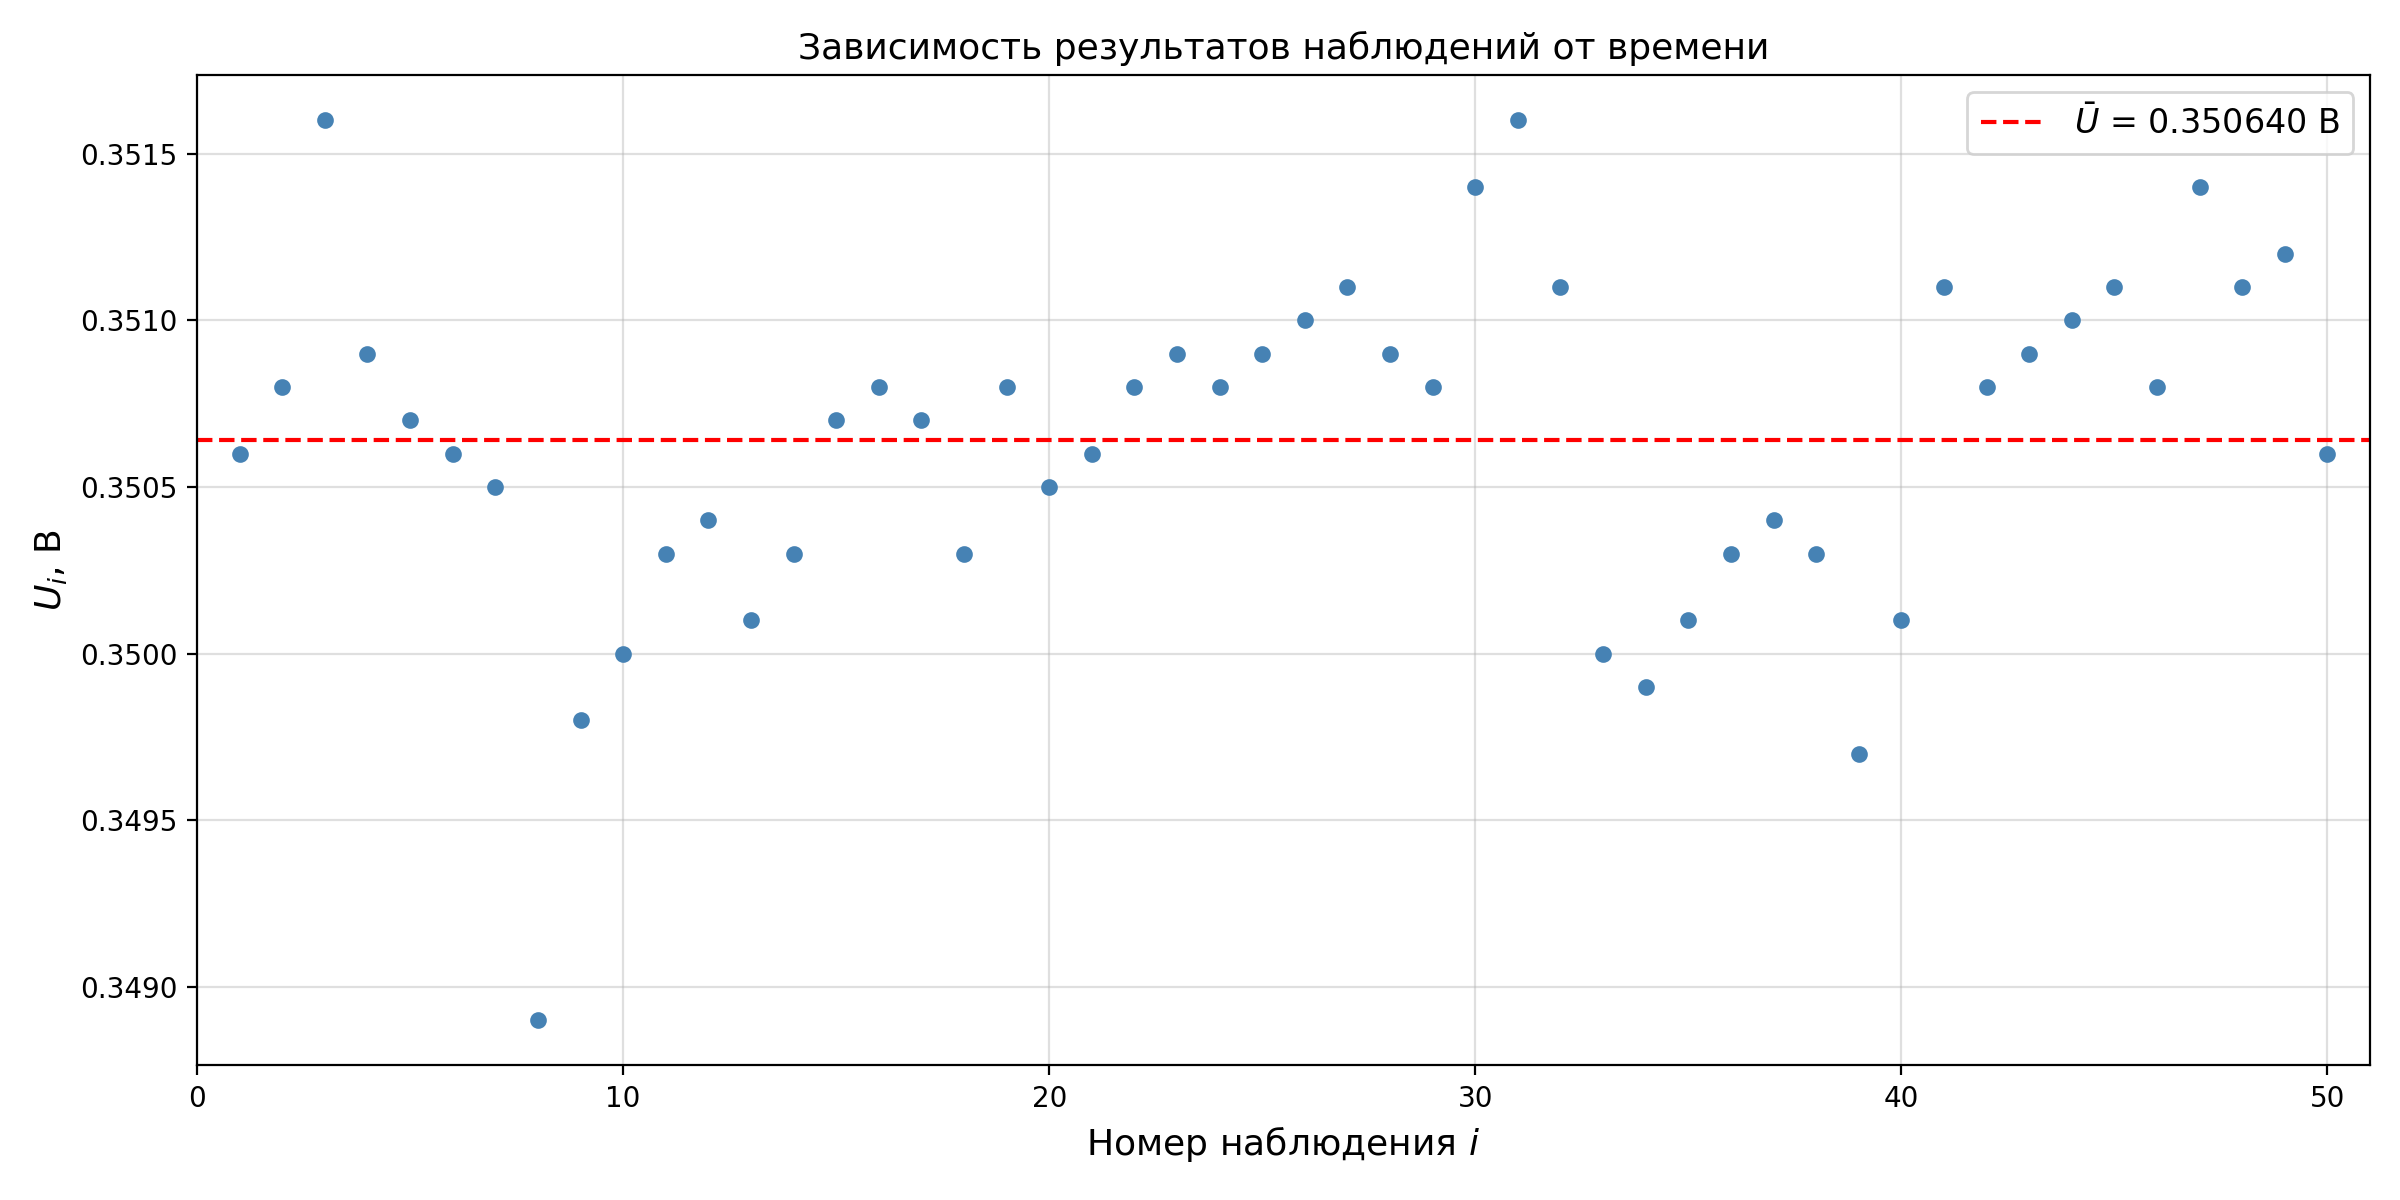
\includegraphics[width=0.85\textwidth]{timeseries.png}
  \caption{Зависимость результатов наблюдений от времени}
  \label{fig:time}
\end{figure}

На рис.~\ref{fig:numline} показано расположение всех результатов на числовой оси.

\begin{figure}[h]
  \centering
  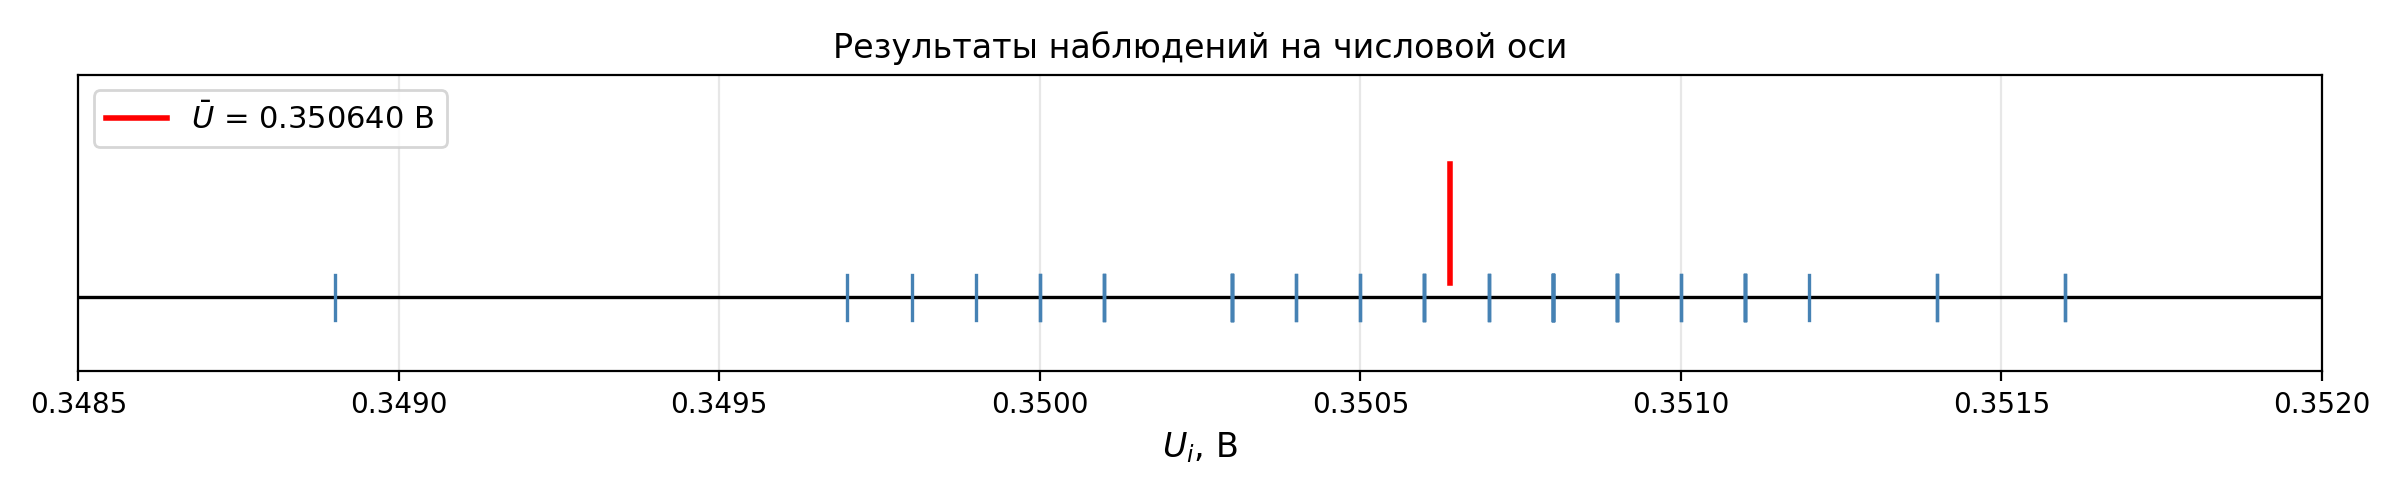
\includegraphics[width=0.85\textwidth]{numberline.png}
  \caption{Результаты наблюдений на числовой оси}
  \label{fig:numline}
\end{figure}

На рис.~\ref{fig:hist} представлены гистограмма и приближённый график
$\Delta n / n = f(U)$. По ширине кривой на уровне $0{,}6$ от максимума
(точки перегиба кривой Гаусса) можно оценить $\sigma \approx 0{,}0005$~В.

\begin{figure}[h]
  \centering
  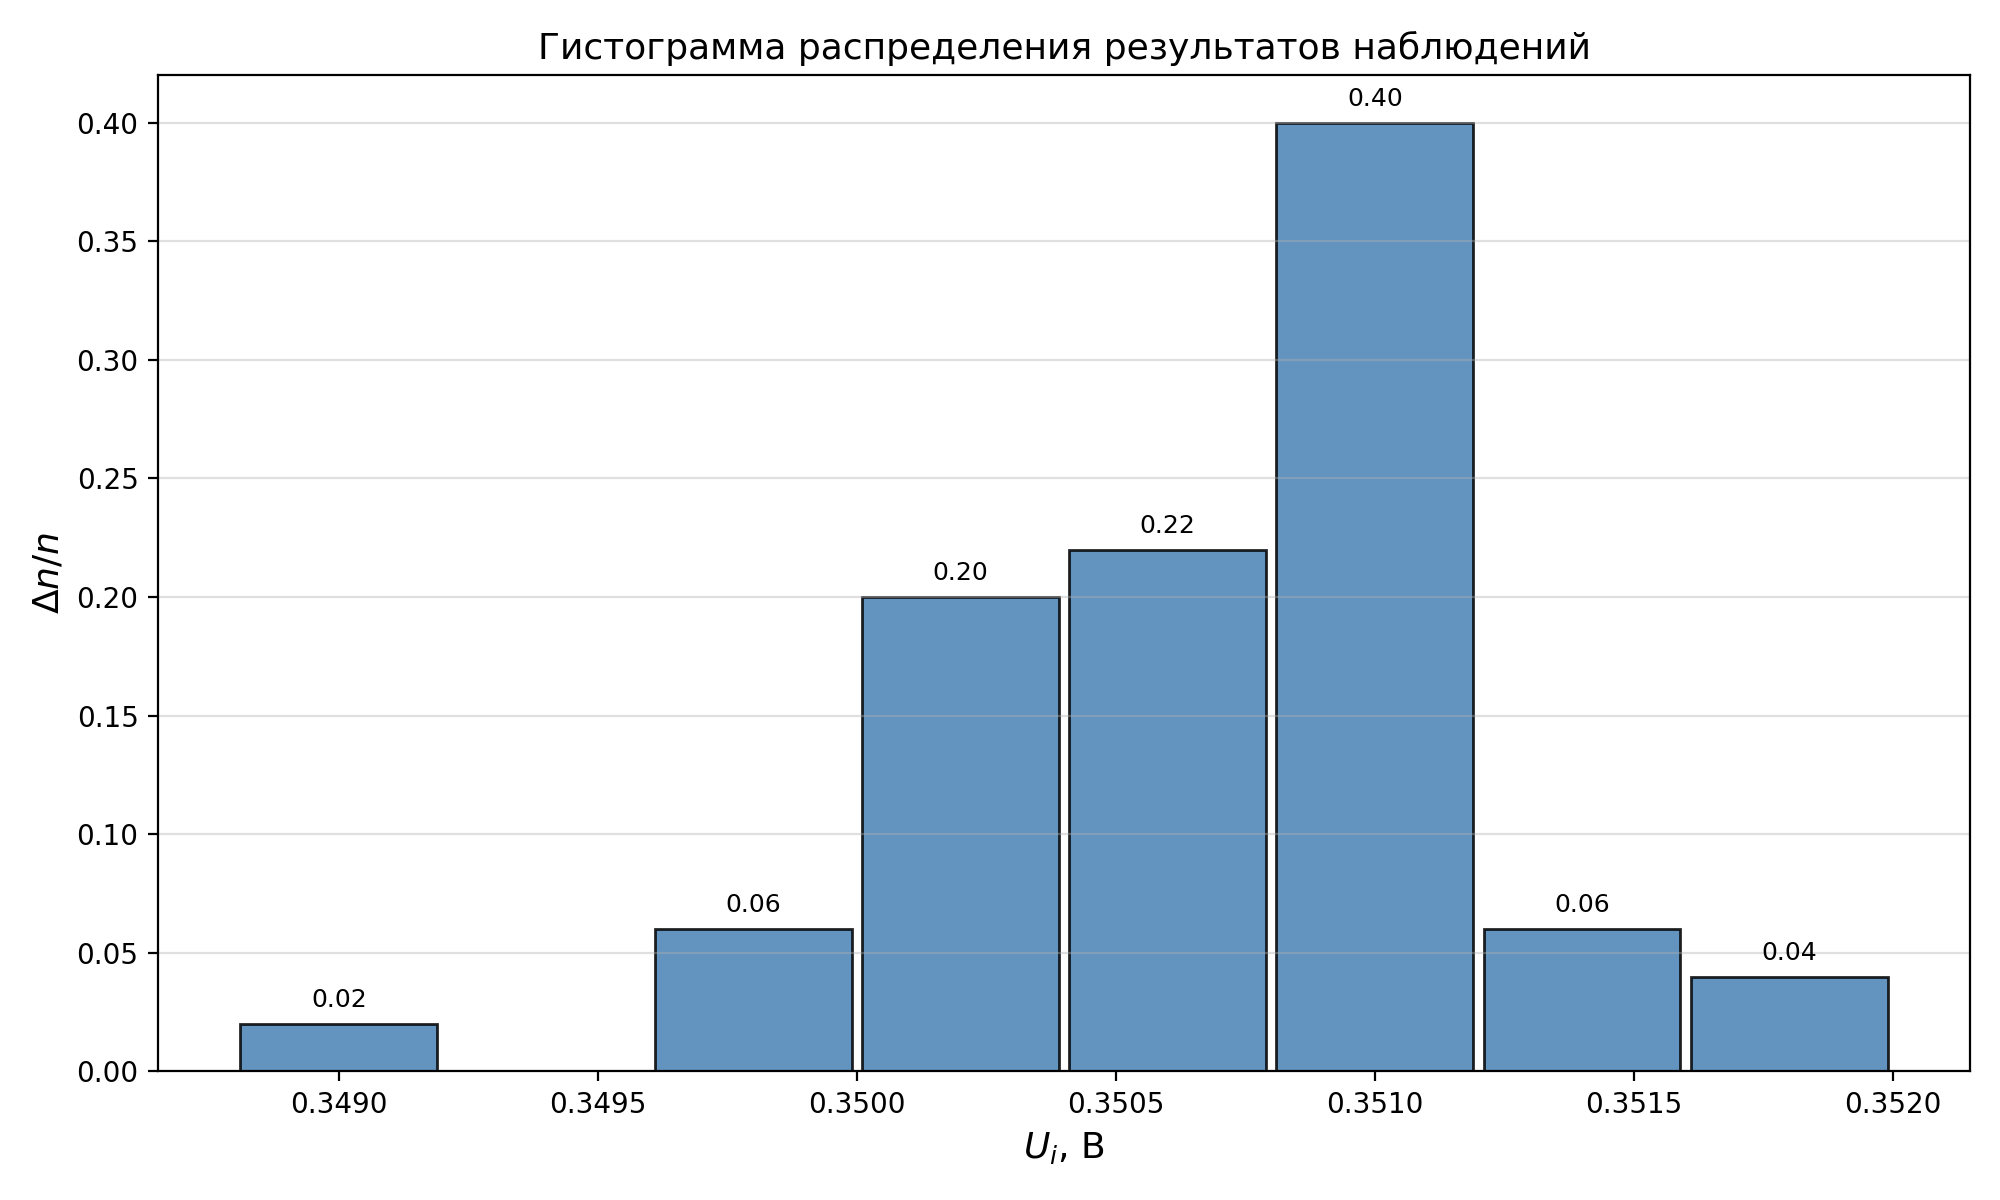
\includegraphics[width=0.78\textwidth]{histogram.png}
  \caption{Гистограмма распределения результатов наблюдений}
  \label{fig:hist}
\end{figure}

\subsubsection{Вычисление погрешностей}

\paragraph{Среднее значение} (формула~\eqref{eq:mean}):
\[
  \bar{U} = \frac{\sum_{i=1}^{50} U_i}{50} = 0{,}35064 \text{ В}.
\]

\paragraph{Стандартная погрешность отдельного наблюдения} (формула~\eqref{eq:s}):
\[
  s = \sqrt{\frac{\sum d_i^2}{n-1}}
    = \sqrt{\frac{1{,}278\times10^{-5}}{49}}
    = 5{,}11\times10^{-4} \text{ В}.
\]

\paragraph{Погрешность среднего} (формула~\eqref{eq:smean}):
\[
  s_{\bar{U}} = \frac{s}{\sqrt{n}}
              = \frac{5{,}11\times10^{-4}}{\sqrt{50}}
              = 7{,}22\times10^{-5} \text{ В}.
\]

\paragraph{Погрешность прибора} (точная шкала $U_K = 1$~В,
формула~\eqref{eq:omega}):
\[
  S = \left(0{,}05 + 0{,}05\cdot\frac{1{,}0}{0{,}35064}\right)\%
    = 0{,}1926\%,
  \qquad
  \omega = 0{,}1926\% \times 0{,}35064\text{ В}
         = 6{,}75\times10^{-4} \text{ В}.
\]

\paragraph{Определение ситуации.}
Сравниваем $s$ и $\omega/3$:
\[
  \frac{\omega}{3} = \frac{6{,}75\times10^{-4}}{3} = 2{,}25\times10^{-4} \text{ В},
  \qquad
  s = 5{,}11\times10^{-4} \approx 2{,}27 \cdot \frac{\omega}{3}.
\]
Так как $s \approx 2{,}3\,(\omega/3)$, имеем \textbf{ситуацию~3}
($\omega/4 \leq s \leq 4\omega$). Суммарная погрешность оценивается
по формуле~(18) из методического пособия:
\[
  s_{\text{сум}} = \sqrt{\left(\frac{\omega}{3}\right)^2 + s_{\bar{U}}^2}
                = \sqrt{(2{,}25\times10^{-4})^2 + (7{,}22\times10^{-5})^2}
                = 2{,}36\times10^{-4} \text{ В}.
\]

\paragraph{Доверительный интервал} при $\alpha = 0{,}95$, $n = 50$:
коэффициент Стьюдента $t_{0{,}95;\,50} = 2{,}01$ (табл.~1, приложение~3 пособия).
\[
  \varepsilon_{0{,}95}
    = t_{\alpha,n} \cdot s_{\bar{U}}
    = 2{,}01 \times 7{,}22\times10^{-5}
    = 1{,}45\times10^{-4} \text{ В}.
\]

%--- 3. Выводы ---
\section{Выводы}

В ходе лабораторной работы было измерено постоянное напряжение цифровым
вольтметром. На грубой шкале (10~В) случайные погрешности не проявлялись —
разброс результатов был меньше единицы последнего разряда. На точной шкале
(1~В) получена выборка из $n = 50$ наблюдений, статистическая обработка которой
позволила получить следующие результаты:

\begin{itemize}
\item среднее значение: $\bar{U} = 0{,}35064$~В;
\item стандартная погрешность отдельного наблюдения: $s = 5{,}1\times10^{-4}$~В;
\item погрешность прибора: $\omega = 6{,}7\times10^{-4}$~В;
\item поскольку $s \approx 2{,}3\,(\omega/3)$, реализована \textbf{ситуация~3},
      суммарная погрешность оценена по приближённой формуле:
      $s_{\text{сум}} = 2{,}4\times10^{-4}$~В.
\end{itemize}

\medskip
\noindent\textbf{Окончательный результат:}
\[
  \boxed{U = (0{,}3506 \pm 0{,}0001) \text{ В} \quad (\alpha = 0{,}95).}
\]

Дрейф измеряемого напряжения в ходе эксперимента не наблюдался. Гистограмма
распределения результатов наблюдений качественно соответствует нормальному
закону. Оценка дисперсии по гистограмме ($\sigma \approx 0{,}0005$~В) согласуется
с расчётным значением $s = 5{,}11\times10^{-4}$~В.

%--- Список литературы ---
\begin{thebibliography}{9}
\bibitem{method}
  Обработка результатов измерений: методическое пособие~/ Кафедра физической
  механики СПбГУ. — СПб, 2026.
\bibitem{lab1}
  Многократные прямые измерения физических величин и обработка результатов
  наблюдений. Работа~1~/ Кафедра физической механики СПбГУ. — СПб, 2026.
\end{thebibliography}

\end{document}
